\subsection{Versuchsaufbau}
\label{sec:Versuchsaufbau}
\begin{figure}
  \centering
  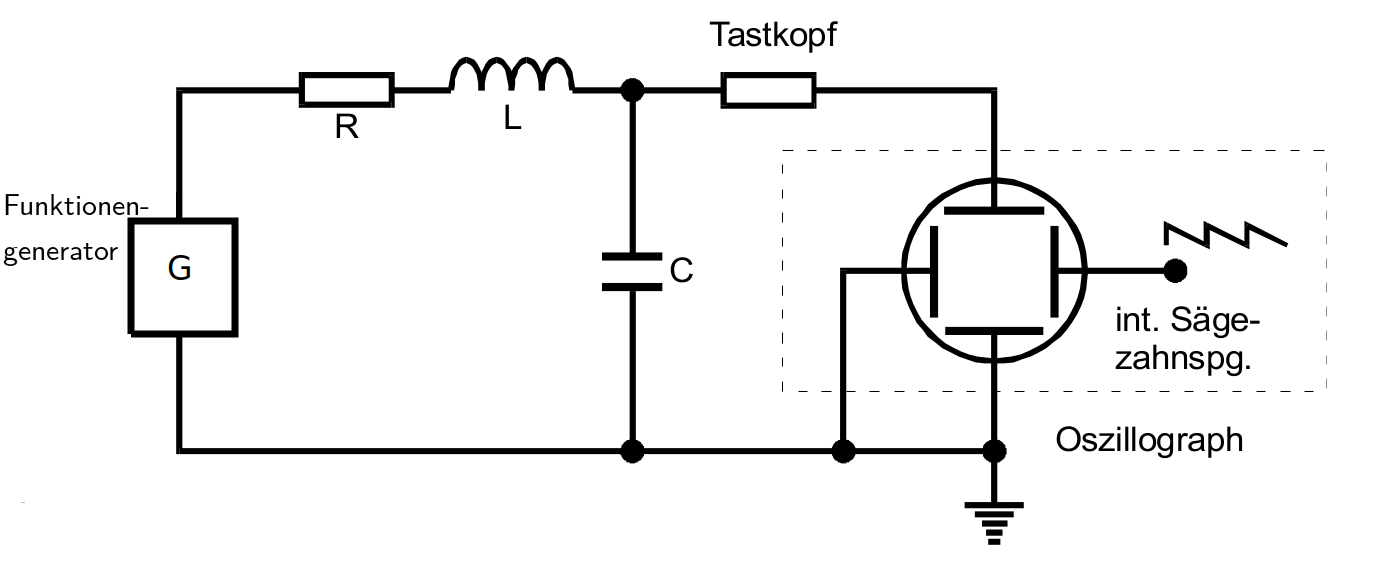
\includegraphics[width=0.75\textwidth]{Bilder/aufbaau.png}
  \caption{Prinzipieller Aufbau des RLC-Schwingkreises zur Untersuchung der zeitabhängigen Spannungsamplitude am Kondensator und des Widerstandes im aperiodischen Grenzfall.}
  \label{fig:aufbau}
\end{figure}
Die Schaltung wird zunächst wie in Abbildung \eqref{fig:aufbau} aufgebaut. Diese besteht aus einem Funktionengenerator, dem RLC-Glied und dem Zweikanal-Oszilloskop mit dem Tastkopf zum Abgreifen der Kondenstaorspannung.
Der Widerstand R kann im vorliegenden Schaltkreis variiert werden. Man hat die Auswahl zwischen drei Widerständen. Die Widerstände $R_\text{1}$ und $R_\text{2}$ sind hierbei fest und der Widerstand $R_\text{3}$ ist als variierbarer Widerstand im Bereich von $0-1000\,\si{\ohm}$ realisiert.
An dem Funktionengenerator lassen sich verschiedene Spannungstypen realisieren. Unter anderem kann dieser verwendet werden, um die verwendete Nadelimpuls-sowie die Sinusspannung zu erzeugen.
Die Größen der Induktivität $L$ und des Kondensators $C$ sind hierbei ebenso bekannt wie die Widerstände $R_\text{1}$ und $R_\text{2}$.
\begin{figure}
  \centering
  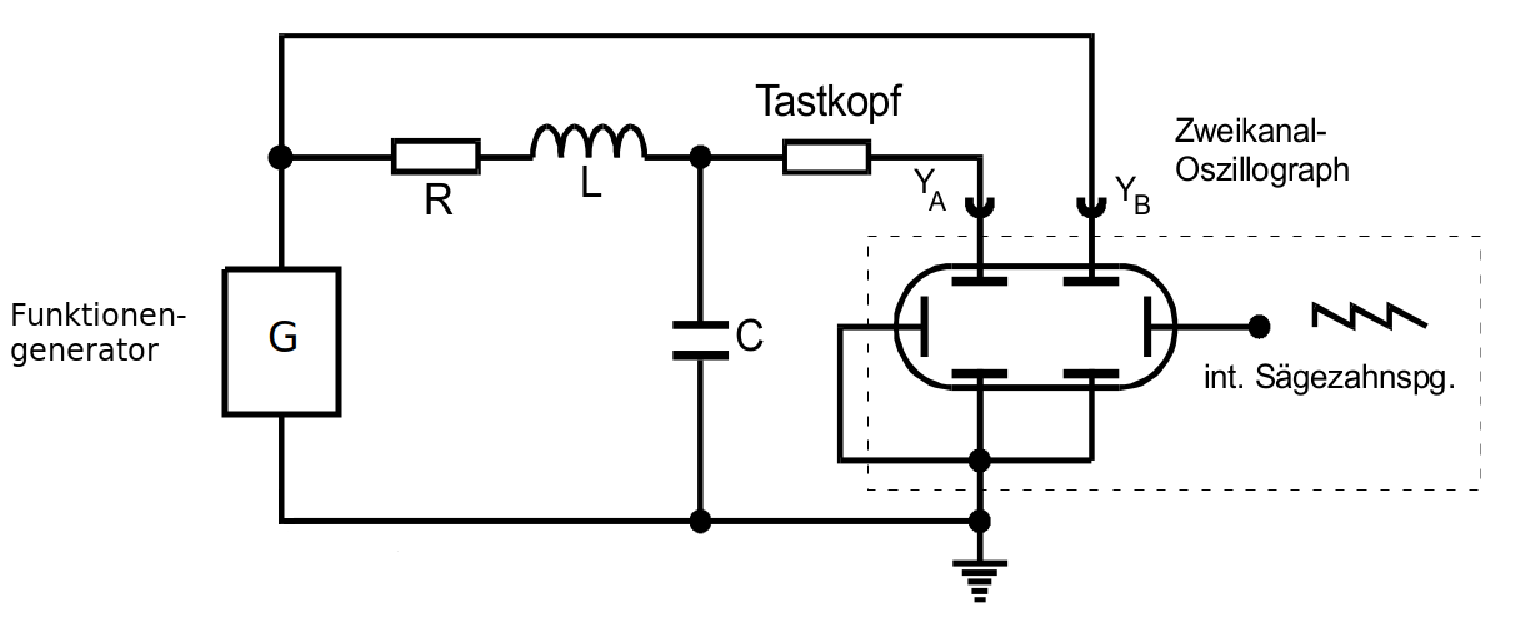
\includegraphics[width=0.75\textwidth]{Bilder/aufbauu.png}
  \caption{Aufbau des RLC-Schwingkreises zur Untersuchung der Frequenzabhängigkeit der Spannungsamplitude und der Phasenverschiebung zwischen Kondensatorspannung und Erregerspannung.}
  \label{fig:aufbau2}
\end{figure}
Zur Messung der Frequenzabhängigkeit der Spannungsamplitude und der Phasenverschiebung zwischen Generatorspannung und Kondensatorspannung wird der Aufbau etwas modifiziert.
Das Zweikanal-Oszilloskop dient nun nicht mehr nur zum Aufzeichnen der Kondensatorspannung sondern der Versuchsaufbau wird wie in Abbildung \eqref{fig:aufbau2} dargestellt, verändert, sodass auf dem zweiten Kanal des Oszilloskops die Generatorspannung aufgenommen wird. Die Generatorspannung und die Kondensatorspannung können nun zugleich am Oszilloskop aufgezeichnet werden.
